\chapter{Post-editing -- what is it?}\label{sec:2}


    \objectives{
        Let us first concentrate on some initial concepts.\\\\
        You will learn...
        
        \begin{itemize}
            \item what PE is, 
            \item who should perform PE tasks,
            \item where and when PE is needed,
            \item about the meaning of MT in professional contexts.
        \end{itemize}
        }

\vspace{\baselineskip}

Before you learn about MT, its development and its different approaches, we want to start with a few thoughts and notions on PE. First, lean back and consider the following questions. You might want to take some notes so that you can take a look at your answers at the end of the discussion and reflect on them.
\begin{itemize}
            \item Have you talked about PE with colleagues? What was their opinion? Did their opinion influence your thoughts on PE?  
            \item How do you think post-editing is different from translation-from-scratch? And how is it different compared to revising translations by colleagues? Do you need similar or different competences for the tasks?
            \item What are your greatest fears when thinking about integrating MT and PE into your professional workflow? What are potential risks?
            \item And how much do you actually know about the functionality of MT and the PE process?
        \end{itemize}

These questions -- amongst many others -- will be discussed in the following chapters. But let's get started at the very beginning. First, we need to define some terms to ensure that we are on the same page. Post-editing (PE) “is the correction of raw machine-translated output by a human translator according to specific guidelines and quality criteria“ \citep[197-198]{obrien_towards_2011}. This definition points out two very important characteristics of post-editing, which we will discuss a little in the following.

\citet{obrien_towards_2011} specifically states that PE should be performed by a human translator and not a layperson who is capable in the source and target language or – even worse – only the target language.\footnote{There are also methods for automatic post-editing, which we, however, will not discuss in further detail. Read \citet{do2020review} for an overview and evaluation of automatic PE methods.} Hence, we can assume that PE has common features with translation – one of the topics we will discuss in the chapter on PE competence (see \sectref{sec:9}). Further, she points out that specific guidelines and quality criteria are important in post-editing similar to the translation brief for human translation jobs. They determine how much post-editing effort is necessary for the respective post-editing job. In a later section, we will discuss different approaches to post-editing and what is essential to each approach. These include the following dichotomies, which we will discuss in the given sections: 
\begin{itemize}
    \item light and full post-editing (see \sectref{sec:4})
    \item monolingual vs. bilingual post-editing (see \sectref{sec:4})
    \item post-editing vs. interactive MT editing (see \sectref{sec:6})
\end{itemize}


\begin{figure}[b]
% 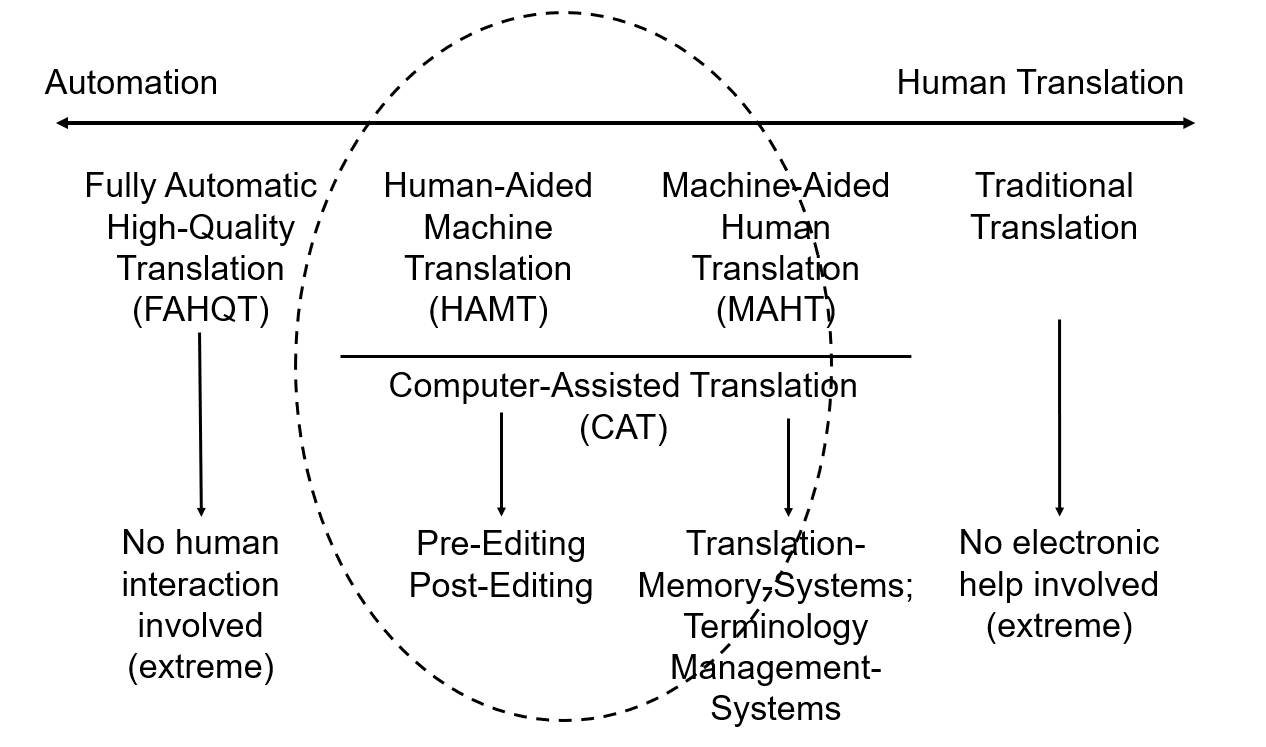
\includegraphics[height=0.45\textheight]{figures/Dimensions of HT and MT.png}
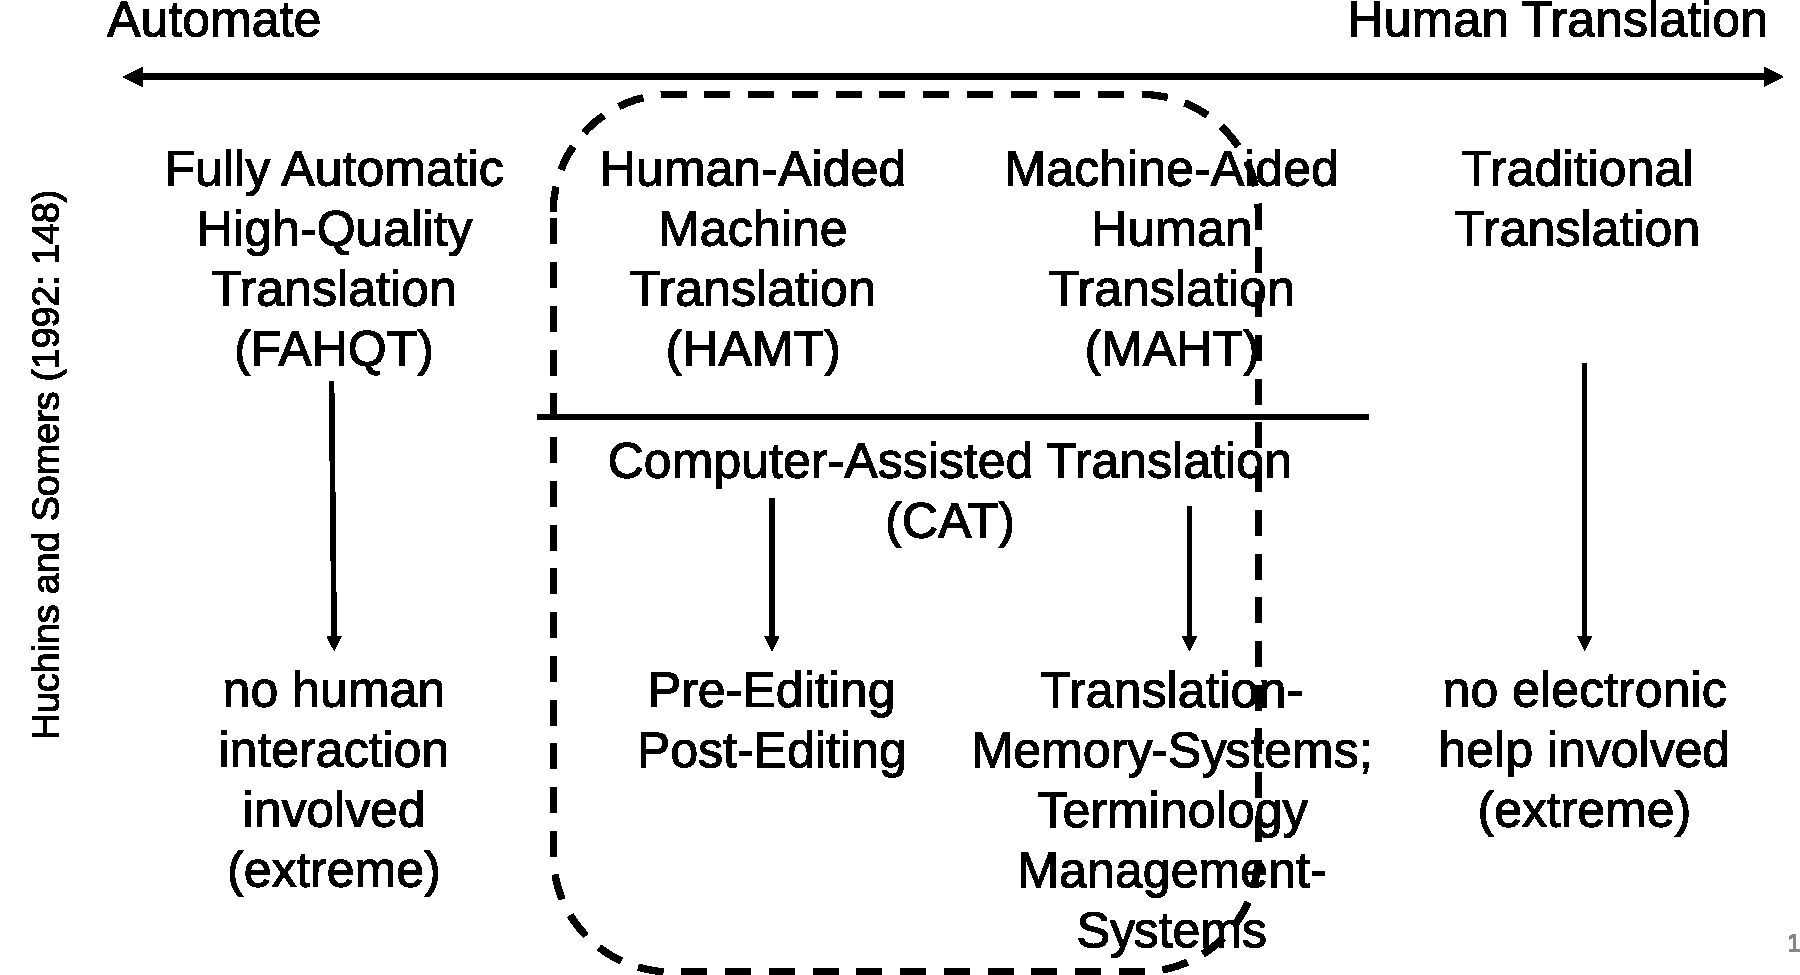
\includegraphics[width=\textwidth]{figures/Dimensions of HT and MT.pdf}
\caption{Dimensions of human and machine translation adapted from \citet[148]{hutchins1992introduction} }
\label{fig:key:2:1}
\end{figure}

As in many other disciplines, buzzwords such as ``digitalisation", ``artifical intelligence" or ``industry 4.0" have also become relevant in translation studies and practice in recent years. In fact, we have been moving towards the automatisation of translation for decades now. We can imagine the automatisation process of translation as a scale. At one end of the scale (in \figref{fig:key:2:1} on the right), we have human translation. The very end of the scale implies that no electronic aids would be involved. The translators would translate using pen and paper, printed dictionaries and the source text document would also be available as a printed version. At the other end of the scale, we find fully-automatic, high-quality machine translation (FAHQMT). So, the human translator would have no involvement in the translation process at all, except for providing the source text to the machine and receiving the target text. We might argue that both extremes are similarly unlikely. Maybe there are some scenarios where humans and machines do not interact in the translation process at all, but those are rather unlikely.\footnote{Of course, this again refers to professional translation practice. Some students still have to write their exams at universities with pen and paper -- the pros and cons of this procedure, however, will not be discussed here. Similarly, there have been scenarios for FAHQT for very restricted text types for decades. See e.g. the Météo system from Canada in \sectref{sec:3:1}.} At the moment, we are somewhere in between both extremes -- and, as mentioned earlier, we have been there for a while now. Since the 1990s, professional translators have been using CAT tools, a term which typically refers to translation memory systems, terminology management systems and project management systems (for a quick introduction, see e.g. \citealt{folaron2010translation}). 
However, the use of word processing programs or electronic/online dictionaries also counts as a step towards automatisation. When those tools are used, we speak of machine-aided human translation (MAHT). The human is still at the centre of the translation process, but is supported by the machine. One further step towards automatisation is what is called human-aided machine translation (HAMT). Here, MT systems are involved and the human ``solely" has to prepare the source text for the machine (pre-editing) and/or improve the MT output (post-editing). The latter is what we will focus on in this book (marked in a dotted line in \figref{fig:key:2:1}). What you have to keep in mind, though, is that MT output is still only a tool for the professional translator (if you do not agree now, you will probably agree after you have finished the book). The focus in pre- and post-editing is more on the machine and a certain amount of the work is performed by the machine. However, the professional translator is still responsible for transforming the MT output into a translation that matches the quality criteria defined for the target text.


%ich weiß nicht, wie ich die Zeile "of HT and MT.png of HT and MT.bb" rauskriege...

As \cite{allen_post-editing_2003} already pointed out, PE introduced a new perspective to translation studies, because translators never really had to deal with ``half-finished" texts before. In PE, the target text does not need to be produced from scratch. The translators already have an outline for the final product. Hence, PE and human translation can be considered different tasks. Further, machine-translated texts have different characteristics than human translations. Therefore, PE cannot be seen as another form of proof-reading either. While some mistakes, like spelling and typing errors, hardly ever occur in MT output, other mistakes, e.g. syntax or lexicon errors, would almost never occur in human translation. Accordingly, there are many interesting questions that must be answered to define the nature of PE. Here, we have only listed a few:
\begin{itemize}
    \item How much MT is acceptable?
    \item How much PE effort is necessary?
    \item How much time (and money) can be saved?
    \item What is the quality of the post-edited target text?
    \item What is the difference from human translation/proof-reading?
\end{itemize}
We will discuss all these questions in the following sections, providing you with a grounded understanding by the time you finish this book.

\bigskip

From a research point of view, post-editing “is a field in which the human translator and the machine meet – as well as the two disciplines Machine Translation and Translation Science” \citep[35]{culo_influence_2014}. Hence, it is very interesting for interdisciplinary research as well. 
Since this book is intended to be a rather practical guidebook, we do not want to go into detail concerning scientific research on post-editing. We just want to say a few words on the importance of research for this subject matter and where you can find relevant literature and databases with empirical PE data.

First of all, we want to clarify that there are some initial approaches to basic theoretical research concerning PE. One promising theory to describe PE phenomena seems to be the relevance-theoretical approach as cognitive and pragmatic aspects are connected. Post-editors are trained professionals who are able to bridge a communicative gap between languages by editing machine translation output situated in the target context. This task is based on well-founded decisions regarding the source text, the intended recipients, the target culture and the post-editing brief. On a cognitive level, relevance theory assumes that MT output should be edited with the least possible effort envisaging efficient and successful communication. \citet{alves2016investigating} discussed relevance-theoretical aspects for PE. The temporal and cognitive effort is ideally reduced during post-editing as translation options are suggested by the MT system, which the post-editor “solely” has to accept, reject or modify. Typically, guidelines are provided for each PE project to support the post-editors’ decision-making process. A rule that often occurs in PE guidelines is that as much of the raw MT output as possible should be retained to make the process fast and efficient. This also has the advantage for the client that the costs for the translation process decrease. On the other side, however, this also means that the recipients are expected to invest more cognitive effort when reading the target texts as the texts are not linguistically and/or stylistically perfect. \citet{carl2019outline} combined relevance theory and the noisy channel model to approach PE theoretically. They propose a “model in which [relevance theory] complements the ‘Noisy Translator Channel’ by adding constraints of causal interrelation between stimulus, context and interpretation, established by the principle of relevance.” \citep[60]{carl2019outline}


In addition to these theoretical considerations, there is a whole range of empirical studies comparing post-editing to translation-from-scratch, addressing the following research questions (of course, this is only a selection): 
\begin{itemize}
    \item How efficient is PE compared to human translation?
    \item Can cognitive effort while post-editing MT be measured?
    \item How good is the quality of post-edited texts? 
    \item Can MT errors be predicted and PE effort be estimated?
    \item Can PE effort be correlated to MT quality?
    \item Are some language pairs more suitable for MT and PE than others?
    \item Which text types, genres and modalities are particularly suitable for post-editing?
    \item Is there a difference in PE performance when comparing students and professionals?
\end{itemize}

From a methodological point of view, most studies rely on a multi-method approach combining eyetracking with keylogging data. In addition, questionnaires describe the metadata with respect to the participants, such as personal data as well as translation and language competence and experience. There is a widely established research database that includes PE and translation data for several language pairs and levels of expertise: the CRITT Translation Process Research Database (CRITT TPR-DB, \citealt{carl2016critt}). This database enables the triangulation of different kinds of data, which in turn sheds light on sequential and parallel cognitive processing activities, reading and writing processes, post-editing and research strategies. If you would like to learn more about the database, the studies and the resulting publications, please consult the following \href{https://sites.google.com/site/centretranslationinnovation/tpr-db}{website}\footnote{last accessed 12 April 2021}.

\newpage

\section*{Crossword puzzle -- chapter 2}

\begin{Puzzle}{12}{15}
|{} |[5]R 	|{} |{}  |{}     |{}  |{}     |{}  |{}    |{}  |{}    |{}   |.
|{} |[6]E   |M  |P |I    |R |I    |C |A   |L |{}    |{} |.
|{} |L   	|{} |{} |{}  |{} |{}    |{} |{}   |{} |{}    |{}   |.
|{} |[7]E   |Y 	|E  |T  |R  |A  |[3]C  |K    |I  |N     |G    |.
|{} |V   	|{} |{} |{} |{} |{} |A |{}   |{} |{}    |{}   |.
|{} |A   	|{} |{} |{} |[4]P |{} |T |{} |{}  |{}     |{}    |.
|{} |N    	|{} |{} |[8]C |R |I    |T |T   |{} |{}    |{}   |.
|{} |C   	|{} |{} |{} |E  |{}  |O  |{}    |{}  |{} |{}    |.
|{} |E   	|{} |{} |{} |E |{}   |O |{}   |{} |{}     |{}   |.
|{} |{}   	|{} |{} |{} |D |{} 	 |L  |{}    |{}  |{}     |{}    |.
|{} |{}   	|{} |{} |{} |I |{}   |S |{}   |{} |{}     |{}   |.
|[2]E  |F   |F  |O |R  |T |{}    |{} |{}   |{} |{}    |{}   |.
|{} |{}   |{}   |{} |{}|I |{}    |{} |{}   |{} |{}    |{}   |.
|{} |{}   |[1]T |R |A    |N |S    |L |A   |T |O    |R   |.
|{} |{}   |{}   |{}|{}   |G |{}    |{} |{}   |{} |{}    |{}   |.
\end{Puzzle}

\begin{PuzzleClues}{\textbf{Across}}
\Clue{1}{TRANSLATOR}{Who should be the post-editor? A professional ...}
\Clue{2}{EFFORT}{Specific guidelines and quality criteria define how much ... a post-editor has to put into the post-editing job.}
\Clue{6}{EMPIRICAL}{What kind of studies exist about post-editing aside from theoretical considerations?}
\Clue{7}{EYETRACKING}{What kind of methodology is often used in cognitive translation studies in addition to keylogging?}
\Clue{8}{CRITT}{What is the name of the Translation Process Research Database?}
\end{PuzzleClues}

\begin{PuzzleClues}{\textbf{Down}}
\Clue{3}{CATTOOLS}{What is the term that refers to translation memory systems, terminology management systems and project management systems?}
\Clue{4}{PREEDITING}{What do we call the preparation of the source text for machine translation?}
\Clue{5}{RELEVANCE}{According to which theory would we assume that MT output should be edited with the least possible effort to achieve the most efficient and successful communication?}
\end{PuzzleClues}
